
% Introduzione +++++++++++++++++++++++++++++++++++++++++++++++++++++++++++++++++

Le equazioni che descrivono i fenomeni fisici hanno carattere tensoriale,
 cioè sono indipendenti dal sistema di coordinate nelle quali vengono scritte.
\'E importante capire la natura tensoriale delle leggi fisiche, capirne
 l'\textbf{invarianza} rispetto ai sistemi di coordinate ed essere in grado di
 scrivere correttamente le equazioni nei sistemi di coordinate più vantaggiosi
 per la descrizione del fenomeno fisico e per la soluzione dei problemi.

\vspace{0.2cm}
\noindent
In questo capitolo verrà usata la notazione di Einstein: è sottointesa la sommatoria
 sugli indici ripetuti in una espressione. Per chiarezza,
\begin{equation}
 a_k b_k = \displaystyle\sum_k a_k b_k .
\end{equation}
%
Si considerano qui solo spazi vettoriali dotati di 
 prodotto interno, per i quali è possibile evitare di introdurre concetti
 più generali, ma più astratti e del tutto inessenziali per una prima
 introduzione ai tensori e al calcolo tensoriale: ad esempio è possibile
 ``schivare'' le definizioni di spazio e base duale (parente di quella che qui
 verrà chiamata \textit{base reciproca}), isomorfismi e altri concetti più
 ``matematici''. Vengono comunque dati alcuni riferimenti per una trattazione esaustiva
 dell'argomento.
\newline \noindent
Nell'introduzione all'algebra tensoriale, si considerano spesso \textbf{basi ortonormali} dello spazio vettoriale. Si ricorda che i vettori di una base ortogonale hanno modulo unitario e sono tra di loro ortogonali.
Si ricorda inoltre che il cambio di base tra due basi ortonormali avviene tramite una matrice di rotazione, matrici ortognoali per le quali l'inversa coincide con la trasposta.
Questa ipotesi limita la validità della trattazione, rendendo non necessari i concetti di \textit{covarianza} e \textit{contravarianza} spesso introdotti nello studio dei tensori. Questa ipotesi verrà leggermente rilassata durante l'introduzione al calcolo tensoriale contenuta nel capitolo \S\ref{sec:calcolo}, estendendo la trattazione ai sistemi di riferimento ortogonali (senza la lunghezza unitaria nei vettori della base), che nascono \textit{naturalmente} quando vengono utilizzati alcuni sistemi di coordinate ``notevoli'', come le coordinate cilindriche e le coordinate sferiche. {\color{blue} Si cercherà di comunque di fornire una trattazione generale, evidenziando in blu le formule valide nel caso di basi ortonormali}.

\noindent
\paragraph{Argomenti della sezione.} Le equazioni della fisica hanno un valore assoluto, indipendente dalla scelta dei sistemi del sistema di riferimento o dalle coordinate usate per descrivere il fenomeno fisico. Vettori e tensori sono gli oggetti matematici che rispecchiano questa invarianza del fenomeno fisico dalla base dello spazio fisico. L'introduzione ai tensori si svolgerà lungo il seguente percorso logico:
\begin{itemize}
 \item si introduce il concetto di invarianza concentrandosi sui vettori: 
\begin{itemize}
    \item un vettore fisico $\bm{v}$, inteso come oggetto invariante, può essere scritto come somma dei prodotti delle sue componenti per i vettori di una base dello spazio, $\bm{v} = v^k \bm{b}_k$;
% \item per ricavare le componenti $v^k$ di un vettore espresso nella base $\{ \bm{b}_k \}_{k=1:N}$, viene introdotto il concetto di base reciproca (o \textit{duale}) $\{ \bm{b}^k \}_{k=1:N}$ e viene ricavato il legame con la base ``di partenza'' $\{ \bm{b}^k \}$;
  \item vengono introdotti i concetti di \textit{covarianza} e \textit{contravarianza}, viene spiegato il significato della posizione degli indici (pedici o apici) di componenti o vettori di una base, e viene ricavato il legame tra oggetti covarianti e contravarianti;
%  \item viene introdotta \textbf{la legge di trasformazione delle componenti del vettore, in seguito a un cambio di base}, che rappresenta l'invarianza dei vettori ed è alla base della definizione classica di vettore fisico e tensore;
\end{itemize}
 \item si introduce il concetto di tensore. In questa introduzione si utilizzeranno i concetti presentati in precedenza sui vettori:
 \begin{itemize}
  \item viene definita la base prodotto, utilizzata per scrivere un tensore in componenti;
  \item vengono introdotte le operazioni sui tensori di somma e moltiplicazione per uno scalare;
%  \item viene ripresa la legge di trasformazione tra oggetti covarianti e contravarianti;
  \item viene ripresa le regole per \textbf{la trasformazione delle componenti in seguito a un cambio di base}, che rappresenta l'invarianza dei tensori e coincide con la \textbf{definizione classica di tensore};
  \item vengono introdotte altre operazioni sui tensori, invarianti anch'esse, il cui risultato è un nuovo tensore.
 \end{itemize}
\end{itemize}

% Prime definizioni ++++++++++++++++++++++++++++++++++++++++++++++++++++++++++++
\vspace{30pt}
\section{Richiami di algebra lineare}
\vspace{10pt}

% Base e Componenti contravarianti ----------------
\begin{definition}[Base e componenti]
Un vettore $\bm{v}$ di uno spazio vettoriale $\mathcal{V}$ può essere rappresentato in una \textbf{base}\footnote{Una base è un insieme minimale di vettori linearmente indipendenti. La dimensione dello spazio vettoriale coincide con il numero di elementi di una sua base.} $\{ \bm{b}_k \}_{k=1:N}$ dello spazio come, 
\begin{equation}
  \bm{v} = v^k \bm{b}_k ,
\end{equation}
 dove gli scalari $v^k$ sono definiti componenti (contravarianti) del vettore $\bm{v}$ rispetto alla base $\{ \bm{b}_k \}_{k=1:N}$.
\end{definition}

Le componenti $v^k$ vengono definite contravarianti, poiché variano seguendo delle trasformazioni ``contrarie'' rispetto a quelle dei vettori di una base $\bm{b}_k$ per garantire l'invarianza del vettore in seguito a un cambio di base, come dettagliato in seguito nel paragrafo \ref{ch:tensori:cambio_base}.

Durante una trattazione generale dell'algebra tensoriale bisogna prestare attenzione alla posizione degli indici usati, poiché questa indica la natura covariante o contravariante degli oggetti. Viene usata la seguente convenzione:
\begin{itemize}
\item gli oggetti \textbf{covarianti} sono indicati con i \textbf{pedici};
\item gli oggetti \textbf{contravarianti} sono indicati con gli \textbf{apici}.
\end{itemize}
%
    I termini \textbf{covariante} e \textbf{contravariante} si riferiscono alla legge di trasformazione dell'oggetto (componenti o vettori della base) al quale sono riferiti, in seguito a un cambiamento della base. In particolare, gli oggetti covarianti sono quelli che seguono la stessa legge di trasformazione degli elementi della base  $\{ \bm{b}_k \}_{k=1:N}$, mentre gli oggetti contravarianti seguono la trasformazione inversa, come si vedrà meglio paragrafo \ref{ch:tensori:cambio_base}. 
% 

Un vettore e tutti gli \textbf{oggetti invarianti} al cambio di sistemi di riferimento (tensori), devono avere componenti contravarianti rispetto agli elementi della base.
% \end{remark}

\begin{definition}[Base duale e componenti covarianti]
Data una base $\{\bm{b}_k\}_{k=1:N}$, i vettori della sua base duale $\{\bm{b}^k\}_{k=1:N}$ sono quei vettori per i quali
\begin{equation}
 \bm{b}^i \cdot \bm{b}_k = \delta^i_k =
 \begin{cases}
   1 \ , \quad i  =   k \\
   0 \ , \quad i \neq k \\
 \end{cases}
\end{equation}
Il vettore $\bm{v}$ può essere espresso nella base covariante, tramite le sue componenti covarianti $v_k$,
\begin{equation}
  \bm{v} = v_k \bm{b}^k \ .
\end{equation}
\end{definition}

\begin{definition}[Simboli $g_{ik}$ e $g^{ik}$]
Si definiscono i simboli $g_{ik}$, $g^{ik}$ come il prodotto scalare dei vettori della base,
\begin{equation}
 g_{ik} := \bm{b}_i \cdot \bm{b}_k  \qquad , \qquad
 g^{ik} := \bm{b}^i \cdot \bm{b}^k \ .
\end{equation}
\end{definition}
%
I simboli $g_{ik}$, $g^{ik}$ possono essere utilizzati per trasformare gli oggetti covarianti in quelli contravarianti e viceversa
\begin{fBox}
\begin{equation}\label{eqn:xxx}
\begin{aligned}
 &  \bm{b}_i = g_{ik} \bm{b}^k  \qquad , \qquad v^i = g^{ik} v_k \\
 &  \bm{b}^i = g^{ik} \bm{b}_k  \qquad , \qquad v_i = g_{ik} v^k
\end{aligned}
\end{equation}
\end{fBox}
%
Come esempio, si dimostra la prima delle (\ref{eqn:xxx}), moltiplicandola scalarmente per il vettore $\bm{b}_q$ della base covariante,
\begin{equation}
 \bm{b}_i \cdot \bm{b}_q = g_{ik} \underbrace{\bm{b}^k \cdot \bm{b}_q}_{=\delta^k_q}  \qquad \rightarrow \qquad \bm{b}_i \cdot \bm{b}_q = g_{iq} \ .
\end{equation}

% ===============================================================
  \subsection{Cambio di base e regole di trasformazione: covarianza e contravarianza.}\label{ch:tensori:cambio_base}
  I termini ``covariante'' o ``contravariante'' sono riferiti alla legge di trasformazione di un oggetto (componente o elemento di una base), se confrontata con la legge di trasformazione degli elementi della base $\{ \bm{b}_k \}_{k=1:N}$ di $\mathcal{V}$.
  Gli apici sono riservati agli oggetti contravarianti (le componenti $v^k$ del vettore $\bm{v}$ e gli elementi della base reciproca $\{ \bm{b}^k \}_{k=1:N}$), mentre i pedici sono riservati agli oggetti covarianti (le componenti $v_k$ del vettore $\bm{v}$ e gli elementi della base $\{ \bm{b}_k \}_{k=1:N}$ di $\mathcal{V}$).
  
\vspace{5pt} \noindent
\textbf{Vettori della base.} Due basi $\{ \bm{b}_k \}_{k=1:N}$ e $\{ \bm{\hat{b}}_k \}_{k=1:N}$ dello spazio vettoriale $\mathcal{V}$ sono legate dalla trasformazione lineare $T$,
\begin{fBox}
\begin{equation}\label{eqn:b2b:t}
  \bm{b}_k = \hat{T}^q_k \bm{\hat{b}}_q \ , \quad \bm{\hat{b}}_k = {T}^q_k \bm{b}_q \ ,
\end{equation}
\end{fBox}
 dove con $\hat{T}$ viene indicata la trasformazione inversa di $T$, $\hat{T} = T^{-1}$. Usando il formalismo matriciale, si può scrivere
\begin{equation}
\begin{aligned}
 \big[ \bm{b}_1 | \dots | \bm{b}_N\big] & =
    \big[ \bm{\hat{b}}_1 | \dots | \bm{\hat{b}}_N\big] \big[ \hat{T}^{q}_{k} \big] =
    \big[ \bm{\hat{b}}_1 | \dots | \bm{\hat{b}}_N\big] \hat{T} , \\
    \big[ \bm{\hat{b}}_1 | \dots | \bm{\hat{b}}_N\big] & =
    \big[ \bm{b}_1 | \dots | \bm{b}_N\big] \big[ T^{q}_{k} \big] =
    \big[ \bm{b}_1 | \dots | \bm{b}_N\big] T
\end{aligned} \qquad \rightarrow \qquad T = \hat{T}^{-1} \ .
\end{equation}
avendo interpretato il pedice della trasformazione $T$ come l'indice di colonna e l'apice come indice di riga.

\vspace{5pt} \noindent
\textbf{Componenti contravarianti.} Le componenti contravarianti $v^k$ di $\bm{v}$ variano secondo la trasformazione inversa degli elementi della base $\{ \bm{b}_k \}_{k=1:N}$ di $\mathcal{V}$,
\begin{fBox}
\begin{equation}\label{eqn:v2v:t}
 \hat{v}^k = \hat{T}^k_q v^q \ , \quad v^k = T^k_q \hat{v}^q \ .
\end{equation}
\end{fBox}
\'E possibile verificare immediatamente le (\ref{eqn:v2v:t}), inserendo la trasformazione (\ref{eqn:b2b:t}) nella rappresentazione del vettore $\bm{v}$ nella base covariante $\{ \bm{b}_k \}_{k=1:N}$,
 \begin{equation}
  \bm{v} = v^q \bm{b}_q = v^q \hat{T}^k_q \bm{\hat{b}}_k = \hat{v}^k \bm{\hat{b}}_k \ .
 \end{equation}

\vspace{5pt} \noindent
\textbf{Trasformazione di cambio base.} La trasformazione di cambio base $\hat{T}$ e della sua inversa $T$ che legano i vettori delle basi $\{\bm{b}_k\}$ e  $\{\bm{b}^k\}$ tramite le formule (\ref{eqn:b2b:t}) hanno l'espressione,
\begin{fBox}
\begin{equation}
  \hat{T}^q_k = \bm{\hat{b}}^q \cdot \bm{b}_k \quad , \quad T^q_k = \bm{b}^q \cdot \bm{\hat{b}}_k \ .
\end{equation}
\end{fBox}
Non è difficile dimostrare queste espressioni. Ad esempio, moltiplicando scalarmente la prima delle (\ref{eqn:b2b:t}) con il vettore $\bm{\hat{b}}^i$, si ottiene
\begin{equation}
 \bm{\hat{b}}^i \cdot \bm{b}_k = \bm{\hat{b}}^i \cdot \left( \hat{T}^q_k \bm{\hat{b}}_q \right)
 \qquad  \rightarrow \qquad 
 \bm{\hat{b}}^i \cdot \bm{b}_k = \hat{T}^q_k \, \delta^i_q = \hat{T}^i_k \ .
\end{equation}

% ===============================================================
\subsection{Vettori e basi ortornomali}
Una base ortonormale $\{\bm{b}_k\}_{k=1:N}$ è una base per la quale i simboli $g_{ik}$ valgono
{\color{blue}
 \begin{equation}
  g_{ik} = \delta_{ik} = 
  \begin{cases}
   1 & i = j \\
   0 & i \ne j \ .
  \end{cases}
 \end{equation}
}
Poiché i simboli $g_{ik}$ sono le componenti di una matrice identità, la base reciproca coincide alla base di riferimento,
{\color{blue}
\begin{equation}
    \bm{b}_k = \bm{b}^k =: \bm{\hat{e}}_k \ ,
\end{equation}
}
così come le componenti covarianti corrispondono alle componenti contravarianti,
{\color{blue}
\begin{equation}
  v^k = v_k = \hat{v}_k \ .
\end{equation}
Nel caso di basi ortonormali, e solo in questo caso, non è indispensabile distinguere oggetti covarianti e contravarianti. Dal punto di vista della notazione, è possibile confondere pedici e apici.
}

\subsubsection{Trasformazione dei vettori di due basi ortonormali}
Le componenti delle trasformazione lineare $\hat{T}$ e della sua inversa $T$ che legano i vettori delle due basi ortonormali $\{\bm{b}_k\}$ e $\{\bm{b}^k\}$ tramite le formule (\ref{eqn:b2b:t}) hanno l'espressione
\begin{fBox}
\begin{equation}
{\color{blue}
  \hat{T}^q_k = \bm{\hat{b}}_q \cdot \bm{b}_k \quad , \quad T^q_k = \bm{b}_q \cdot \bm{\hat{b}}_k \ .
}
\end{equation}
\end{fBox}
Per verificare queste formule è sufficiente usare il prodotto scalare con i vettori della base reciproca. Infatti,
{\color{blue}
\begin{equation}
\begin{aligned}
 \bm{b}_k & = \hat{T}^i_k \bm{\hat{b}}_i \qquad , \qquad 
 \bm{\hat{b}}_q \cdot \bm{b}_k = \hat{T}^i_k \underbrace{\bm{\hat{b}}_q \cdot \bm{\hat{b}}_i}_{=\delta^q_i} \quad \rightarrow  \quad \hat{T}^q_k = \bm{\hat{b}}_q \cdot \bm{b}_k \\
 \bm{\hat{b}}_k & = {T}^i_k \bm{b}_i \qquad , \qquad 
 \bm{b}_q \cdot \bm{\hat{b}}_k = T^i_k \underbrace{\bm{b}_q \cdot \bm{b}_i}_{=\delta^q_i} \quad \rightarrow  \quad T^q_k = \bm{b}_q \cdot \bm{\hat{b}}_k \ .
\end{aligned} 
\end{equation}
}
Dal confronto diretto delle due espressioni di $\hat{T}^q_k$ e $T^q_k$, si osserva che la trasformazione inversa $\hat{T}:=T^{-1}$ è uguale alla matrice trasposta $T^T$ della matrice di cambiamento di base $T$,
{\color{blue}
\begin{equation}
 \hat{T} := T^{-1} = T^T \qquad , \qquad \hat{T}^q_k = T^k_q \ .
\end{equation}
}

%%% Dimostriamo ora che le trasformazioni che legano i vettori di due basi ortonormali sono delle rotazioni.\footnote{In generale la trasformazione che lega due basi ortogonali è un'isometria, cioè una trasformazione a determinante unitario. Le ismometrie possono essere rotazioni o riflessioni. Le uniche isometrie che conservano l'orientamento dello spazio sono le rotazioni, trasformando ad esempio una base destrorsa in un'altra base destrorsa.}
%%%  Valgono le regole generali (\ref{eqn:b2b:t}) e (\ref{eqn:b2b:ti}) di trasformazione degli elementi delle basi di riferimento e reciproche,
%%%  \begin{equation}
%%%  \begin{aligned}
%%%      \bm{b}_i  = \tilde{T}^k_i \tilde{\bm{b}}_k \quad & ,  \quad \tilde{\bm{b}}_i  =         T^k_i  \bm{b}_k \\
%%%  \end{aligned}
%%%  \end{equation}
%%% %
%%% Sfruttando l'uguaglianza delle basi di riferimento con le loro basi reciproche,
%%%  \begin{equation}
%%%      \bm{b}^i = \bm{b}_i = \tilde{T}^k_i \tilde{\bm{b}}_k = \tilde{T}^k_i \tilde{\bm{b}}^k = T^k_i T^k_l \bm{b}^l \ .
%%%  \end{equation}
%%% % La formula qui sopra è stata ottenuta usando le trasformazioni generali e l'uguaglianza delle basi per sistemi di coordinate cartesiane.
%%%   Per trovare quali caratteristiche deve avere la trasformazione $\tilde{T}$, possiamo riscrivere il termine di partenza come $\bm{b}^i = \delta_l^i \bm{b}^l$. Da un confronto del termine così riscritto con l'ultimo termine della formula, si ricava
%%%   \begin{equation}
%%%       \tilde{T}^k_i \tilde{T}^k_l  = \delta_i^l \qquad \rightarrow \qquad
%%%       \tilde{T}_{ki} \tilde{T}_{kl}  = \delta_{li} \qquad \rightarrow \qquad
%%%       \tilde{T}^T \tilde{T} = I
%%%   \end{equation}
%%%   avendo considerato gli apici come i primi indici della trasformazione e quindi come gli indici di riga della matrice $\tilde{T}$ (è analogo considerare gli indici invertiti, ottenendo una definizione di $\tilde{T}$ trasposta). \'E immediato osservare che 
%%% \begin{equation}
%%%   \tilde{T}^T = \tilde{T}^{-1} =: T \qquad \rightarrow \qquad
%%%   \tilde{T}_{ik} = T_{ki} \ .
%%% \end{equation}
%%%   Abbiamo ottenuto quello che volevamo dimostrare, cioè che la trasformazione $\tilde{T}$ che lega due sistemi di coordinate ortonormali è un'\textbf{isometria}: una \textbf{rotazione} se ha determinante =\,1 e conserva l'orientamento dello spazio, una \textbf{riflessione} se ha determinante =\,-1 e trasforma una terna destrorsa in una terna sinistrorsa invertendo l'orientamento dello spazio.

% 
% ##############################################################
%
% \vspace{30pt}
% \noindent
% \begin{tabular}{cc}
% \begin{minipage}{0.98\textwidth}
% \begin{exercise}[Cambio di base]\label{exa:basis}
% \end{exercise}
% \end{minipage}
% \end{tabular}

% ##############################################################
% Definizione di secondo spazio duale V**, isomorfismo canonico tra V e V**: conseguenze pratiche ...
%    ...
\newpage \clearpage
\section{Algebra multilineare}
Le leggi di trasformazione degli elementi di basi differenti e delle relative componenti sono state introdotte per i vettori nella sezione precedente. In questa sezione verranno utilizzate per ottenere le leggi di trasformazione degli elementi della base e delle componenti dei tensori. In particolare, la definizione classica di tensore come oggetto invariante al cambio di sistema di riferimento, coinvolge direttamente la legge di trasformazione delle componenti, in seguito a un cambio di base. L'esempio \ref{exa:basis} è stato pensato come un'occasione per riprendere dimestichezza con l'analisi lineare e prendere familiarità con le definizioni introdotte nel paragrafo.

Se l'algebra lineare è la branca della matematica che si occupa dello studio dei vettori, degli spazi vettoriali (o spazi lineari) e delle trasformazioni lineari, l'algebra multilineare si occupa dello studio dei tensori, degli spazi tensoriali e delle trasformazioni multilineari.

Un tensore può essere definito in maniera intrinseca come una funzione multi-lineare o in maniera classica come un oggetto matemtaico formato da un insieme di numeri, le sue componenti, che seguono delle precise leggi di trasformazione in seguito a un cambio di base, utilizzato per descrivere in maniera astratta e invariante le leggi della fisica.
Viene solo riportata per completezza la definizione intrinseca, dopodiché si ``ricaverà'' la definizione classica di tensore, partendo dalla sua invarianza al cambio di base. 
% Definizione di tensore come funzione multilineare (p,q)
\begin{definition}[Tensore (definizione intrinseca)]\label{def:tensIntrinseca}
 Un tensore di ordine $r$ su $\mathcal{V}$ è una funzione
 $r$-lineare
\begin{equation}
   T : \underbrace{\mathcal{V}   \times \dots \times \mathcal{V}  }_{\text{r volte}} \rightarrow K
%  \qquad \qquad  ( T : \mathcal{V}^r \rightarrow K)
\end{equation}
%
\begin{remark}
 La definizione di tensore data è riferita agli spazi dotati di prodotto interno. Per una prima introduzione all'algebra e al calcolo tensoriale, può essere considerata un buon compromesso tra comprensibilità e completezza della trattazione, per un corso di ingegneria. Senza voler entrare nei particolari, questa definizione evita di introdurre le definizioni di spazio duale e di isomorfismi necessarie a una trattazione generale dei tensori su spazi vettoriali qualsiasi.
\end{remark}
%
  Si indica con $\mathcal{T}^r(\mathcal{V})$ l'insieme dei tensori di ordine $r$. Questo insieme è chiuso\footnote{Un insieme $\mathcal{V}$ è chiuso rispetto a un'operazione se l'operazione su ogni elemento di $\mathcal{V}$ restituisce un elemento di $\mathcal{V}$.} rispetto alle operazioni di somma e moltiplicazione per uno scalare definite in seguito, e quindi è definito lo spazio vettoriale dei tensori di ordine $r$. %, operazioni rispetto alle quali uno spazio vettoriale deve essere chiuso) 
 Un tensore di ordine $0$ è uno scalare, un tensore di ordine $1$ un vettore.
\end{definition}


\subsection{Prodotto tensoriale tra vettori}
Per arrivare alla definizione classica di un tensore senza introdurre complicazioni superflue per una prima introduzione all'algebra tensoriale, occorre introdurre l'operazione di prodotto tensoriale tra vettori. Questa operazione è la prima operazione incontrata che dà origine a tensori di ordine maggiore di uno (i vettori possono essere considerati tensori di ordine 1).

\begin{definition}[Prodotto tensoriale tra vettori] Dati r vettori $\bm{v}_1,\dots,\bm{v}_r \in \mathcal{V}$ si definisce il loro prodotto tensoriale come il tensore di ordine $r$, indicato con
\begin{equation}
    \bm{v}_1 \otimes \bm{v}_2 \otimes \dots \otimes \bm{v}_r \qquad \text{ o come } \qquad  \bm{v}_1 \bm{v}_2 \dots \bm{v}_r  \ .
\end{equation}
 Se $\mathcal{V}$ è uno spazio vettoriale di dimensione $N$, il prodotto tensoriale di $r$ vettori appartenenti a $\mathcal{V}$ ha dimensioni $N^r$.
\end{definition}
La definizione di prodotto tensoriale tra vettori viene usata per definire una base dello spazio dei tensori di ordine $r$ e ottenere una rappresentazione per componenti di un tensore. In seguito verrà definito anche il prodotto tensoriale tra tensori di ordine qualsiasi. 
\begin{remark}
 Il prodotto tensoriale \textbf{non è commutativo}, $\bm{a} \otimes \bm{b} \neq \bm{b} \otimes \bm{a}$.
\end{remark}

\subsection{Base prodotto e componenti di un tensore}
Per rappresentare in componenti un tensore di ordine $r$ è necessario definire una base dello spazio dei tensori $\mathcal{T}^r(\mathcal{V})$. Ad esempio, data una base $\{ \bm{b}_k \}$ dello spazio $\mathcal{V}$, è possibile definire la base prodotto tramite il prodotto tensoriale degli elementi della base.
\begin{definition}[Base prodotto di $\mathcal{T}^r(\mathcal{V})$] %Se lo spazio $\mathcal{V}$ ha dimensione $N$, la dimensione dello spazio $\mathcal{T}^r(\mathcal{V})$ è $N^r$.
 La base $\{ \bm{b}_k \}_{k=1:N}$ di $\mathcal{V}$
    induce una base prodotto (covariante) di $\mathcal{T}^r(\mathcal{V})$, i cui elementi sono formati da tutti i possibili $N^r$ prodotti tensoriali di ordine $r$ dei vettori $\bm{b}_k$
\begin{equation}
  \left\{ \bm{b}_{i_1} \otimes \dots \otimes \bm{b}_{i_r} \right\}_{
  i_1,\dots,i_r = 1 : N} \ ,
\end{equation}
dove tutti gli indici $i_k$ possono variare in maniera indipendente da $1$ a $N$.
\end{definition}

\begin{example}
 La base prodotto dei tensori di ordine $r=2$ nello spazio tridimensionale, $N=3$, indotta dalla base $\{ \bm{b}_1, \bm{b}_2, \bm{b}_3 \}$, è la base formata dai $N^r = 9$ prodotti tensoriali
\begin{equation}
\begin{aligned}
 \{ & \bm{b}_1 \otimes \bm{b}_1 , \  \bm{b}_1 \otimes \bm{b}_2 , \  \bm{b}_1 \otimes \bm{b}_3 , \\
    & \bm{b}_2 \otimes \bm{b}_1 , \  \bm{b}_2 \otimes \bm{b}_2 , \  \bm{b}_2 \otimes \bm{b}_3 , \\
    & \bm{b}_3 \otimes \bm{b}_1 , \  \bm{b}_3 \otimes \bm{b}_2 , \  \bm{b}_3 \otimes \bm{b}_3  \} \ .
\end{aligned}
\end{equation}
\end{example}

\noindent
 Rispetto alla base prodotto, un tensore $\bm{A} \in \mathcal{T}^r(\mathcal{V})$ viene scritto come
 \begin{equation}
  \bm{A} = A^{i_1 \dots i_r} \bm{b}_{i_1} \otimes \dots \otimes \bm{b}_{i_r} ,
 \end{equation}
 dove $A^{i_1 \dots i_r}$ sono le componenti contravarianti del tensore $\bm{A}$ rispetto alla base prodotto covariante.

\paragraph{Base covariante, mista e natura degli indici.}
Come già visto per i vettori, è possibile utilizzare i simboli $g_{ik}$ e $g^{ik}$ per passare dai vettori di una base a quelli della sua duale, e trasformare le componenti contravarianti in quelle covarianti, e viceversa. Si può ripetere lo stesso procedimento per i vettori che formano una base prodotto e ottenere le componenti di un tensore con singoli indici di natura diversa,
\begin{equation}
\begin{aligned}
 \bm{A} & = A^{ijk} \bm{b}_i \otimes \bm{b}_j \otimes \bm{b}_k = & \hspace{1.5cm} ( \quad \bm{b}_i = g_{il} \bm{b}^l \quad ) \\
        & = \underbrace{A^{ijk} \big(g_{il} }_{=: A_l^{\, jk}} \bm{b}^l \big) \otimes \bm{b}_j \otimes \bm{b}_k = A_l^{\, jk} \bm{b}^l \otimes \bm{b}_j \otimes \bm{b}_k \ ,
\end{aligned}
\end{equation}
avendo sostituito solo il primo vettore della base prodotto e, di conseguenza, cambiato la natura del prmo indice delle componenti. Lo stesso procedimento può essere ripetuto per qualsiasi elemento della base prodotto, riassumendo la regola di trasformazione della natura delle componenti tramite l'uso di $g_{ik}$,
\begin{equation}
 A_{l}^{\, jk} = g_{il} A^{ijk} \qquad , \qquad  A^{l}_{\, jk} = g^{il} A_{ijk} \ .
\end{equation}
\begin{remark}
  \'E fondamentale l'ordine degli indici che rappresentano le componenti del tensore. Variando il primo elemento della base prodotto, viene cambiata la natura del primo indice e quindi sarà il primo indice ``ad alzarsi'' o ``ad abbassarsi'' in seguito a questa operazione.
\end{remark}
\begin{remark}
 Si possono ricordare facilmente queste regole, facendo un ``bilancio degli indici'' e ricordando che gli indici ripetuti vengono saturati da una somma. Gli indici che vengono saturati devono comparire uno come apice e uno come pedice. Dalle due parti dell'uguale devono essere presenti gli stessi indici non saturati nelle stesse posizioni, se non si scrivono esplicitamente gli elementi della base e quindi si sottoindende di riferirsi alla stessa base.
\end{remark}

 \subsection{Alcune operazioni tensoriali (I): somma e moltiplicazione per uno scalare.}\label{ch:tensori:operazioniI}
 Le due operazioni di somma e moltiplicazione per uno scalare e la chiusura dell'insieme $\mathcal{T}^r$ rispetto ad esse sono condizioni necessarie alla struttura di spazio vettoriale. La somma di due tensori di ordine $r$ $\bm{A},\bm{B} \in \mathcal{T}^r(\mathcal{V})$ ha come risultato il tensore di ordine $r$ che ha come componenti la somma delle componenti di $\bm{A}$ e $\bm{B}$,
\begin{equation}\label{eqn:tens:somma}
 \bm{A}+\bm{B} = 
    ( A^{i_1 \dots i_r} + B^{i_1 \dots i_r}  ) \bm{b}_{i_1} \otimes \dots \otimes \bm{b}_{i_r}
\end{equation}
 e la moltiplicazione di $\bm{A}$ per uno scalare $\alpha \in K$ ha come risultato un tensore dello stesso ordine, le cui componenti sono il prodotto di $\alpha$ per le componenti di $\bm{A}$, 
\begin{equation}\label{eqn:tens:moltScal}
  \alpha \bm{A} = 
    \alpha A^{i_1 \dots i_r} \bm{b}_{i_1} \otimes \dots \otimes \bm{b}_{i_r} \ .
\end{equation}
%
\vspace{15pt}
\begin{definition}[Spazio vettoriale $\mathcal{T}^r(\mathcal{V})$ dei tensori di ordine $r$] Lo spazio vettoriale $\mathcal{T}^r(\mathcal{V})$ dei tensori di ordine $r$ sullo spazio $\mathcal{V}$ è formato dall'insieme $\mathcal{T}^r(\mathcal{V})$, con le operazioni di somma e moltiplicazione per uno scalare definite in (\ref{eqn:tens:somma}) e (\ref{eqn:tens:moltScal}).
\end{definition}

\subsection{Prodotto tensoriale tra tensori}
\'E possibile ora definire il prodotto tensoriale tra due (o più tensori) di qualsiasi ordine.
\begin{definition}[Prodotto tensoriale]
 Il prodotto tensoriale di due tensori $\bm{A} \in \mathcal{T}^p(\mathcal{V})$, $\bm{B} \in \mathcal{T}^r(\mathcal{V})$ è il tensore di ordine $p+r$ definito come
\begin{equation}
 \bm{A}\otimes\bm{B} = 
   A^{i_1 \dots i_p} B^{j_1 \dots j_r} \bm{b}_{i_1} \otimes \dots \otimes \bm{b}_{i_p}
    \otimes \bm{b}_{j_1} \otimes \dots \otimes \bm{b}_{j_r} \ .
\end{equation}
\end{definition}

 \noindent
 \begin{remark}
     Il prodotto tensoriale \textbf{non è commutativo}: $\bm{A} \otimes \bm{B} \neq \bm{B} \otimes \bm{A}$.
 \end{remark}

%

%  \section{Spazio dei tensori di ordine r $\mathcal{T}^r(\mathcal{V})$}
% L'insieme dei tensori di ordine $r$ costituisce uno spazio vettoriale, indicato con $\mathcal{T}^r(\mathcal{V})$,
% una volta definite le operazioni chiuse di somma e di moltiplicazione per uno scalare.
 
%
% \noindent
%  Si dimostra che le componenti $A^{i_1 \dots i_r}$ sono
%  \begin{equation}
%    A^{i_1 \dots i_r} = \bm{A}(\bm{b}^{i_1},\dots,\bm{b}^{i_r}) .
%  \end{equation}
%  Infatti,
%  \begin{equation}
%  \begin{aligned}
%    \bm{A}(\bm{b}^{k_1},\dots,\bm{b}^{k_r}) & =
%      A^{i_1 \dots i_r} \bm{b}_{i_1} \otimes \dots \otimes \bm{b}_{i_r} ( \bm{b}^{k_1}, \dots, \bm{b}_{l_r})  = \\ & =
%      A^{i_1 \dots i_r} ( \bm{b}_{i_1} \cdot \bm{b}^{k_1} ) \dots (\bm{b}_{l_r} \cdot \bm{b}^{j_r} )  = \\
%      & = A^{i_1 \dots i_r} \delta^{k_1}_{i_1} \dots \delta^{j_r}_{l_r} = A^{k_1 \dots k_r}
%  \end{aligned}
%  \end{equation}

%  le componenti di un tensore $\bm{A} \in \mathcal{T}^p_q(\mathcal{V})$ sono $N^(p+q)$ scalari 
% definiti come
%\begin{equation}
%  A^{i_1 \dots i_p}_{\ \ \ j_1 \dots j_q} = \bm{A}(\bm{b}^{i_1},\dots,\bm{b}^{i_p},\bm{b}_{j_1},\dots,\bm{b}_{j_q})
%\end{equation}
% e il tensore $\bm{A}$ può esere scritto in componenti come
%\begin{equation}
%  \bm{A} = A^{i_1 \dots i_p}_{\ \ \ j_1 \dots j_q} \bm{b}_{i_1} \otimes \dots \otimes \bm{b}_{i_p} \otimes
%   \bm{b}^{j_1} \otimes \dots \otimes \bm{b}^{j_q}
%\end{equation}
 
 \subsection{Cambio di base e regola di trasformazione delle componenti: definizione ``classica'' di tensore.} 
%
 Aiutandosi con la legge di trasformazione (\ref{eqn:b2b:t}) degli elementi della base $\{ \bm{b}_k \}_{k=1:N}$ di $\mathcal{V}$ e della base reciproca $\{ \bm{b}^k \}_{k=1:N}$ di $\mathcal{V}^*$, si può verificare  che la base prodotto (covariante) dello spazio $\mathcal{T}^r(\mathcal{V})$ si trasforma secondo
\begin{fBox}
\begin{equation}\label{eqn:bp2bp:t}
\begin{aligned}
 &  \bm{\hat{b}}_{i_1} \otimes \dots \otimes \bm{\hat{b}}_{i_r} = 
  T^{k_1}_{i_1}\dots T^{k_p}_{i_r}
  \bm{b}_{k_1} \otimes \dots \otimes \bm{b}_{k_r} \\
  &  \bm{b}_{i_1} \otimes \dots \otimes \bm{b}_{i_r} = 
  \hat{T}^{k_1}_{i_1}\dots \hat{T}^{k_r}_{i_r}
  \bm{\hat{b}}_{k_1} \otimes \dots \otimes \bm{\hat{b}}_{k_r} .
\end{aligned}
\end{equation}
\end{fBox}
 Per ricavare la regola di trasformazione della base prodotto (\ref{eqn:bp2bp:t}) è sufficiente applicare la (\ref{eqn:b2b:t}) a tutti i vettori $\bm{b}_{i_\alpha}$ della base prodotto.  Usando la multilinearità del prodotto tensoriale
 \begin{equation}
 \begin{aligned}
  \bm{\hat{b}}_{i_1} \otimes \dots \otimes \bm{\hat{b}}_{i_r} = &
  ( T^{k_1}_{i_1}\bm{b}_{k_1} ) \otimes \dots \otimes ( T^{k_p}_{i_r}\bm{b}_{k_r}) = \\
  = & T^{k_1}_{i_1}\dots T^{k_r}_{i_r}
   \bm{b}_{k_1} \otimes \dots \otimes \bm{b}_{k_r} . \\
 \end{aligned}
 \end{equation}
%
 La regola di trasformazione delle componenti di un tensore $\bm{A} \in \mathcal{T}^r(\mathcal{V})$, $\bm{A} =$ $A^{i_1 \dots i_r} \bm{b}_{i_1} \otimes \dots \otimes \bm{b}_{i_r} =$ $\hat{A}^{i_1 \dots i_r} \bm{\hat{b}}_{i_1} \otimes \dots \otimes \bm{\hat{b}}_{i_r} $ al variare dei sistemi di riferimento è
\begin{fBox}
\begin{equation}\label{eqn:t2t:t}
\begin{aligned}
 &  \hat{A}^{k_1 \dots k_r} = 
  \hat{T}^{k_1}_{i_1}\dots \hat{T}^{k_r}_{i_r} A^{i_1 \dots i_r} \\
 &  A^{i_1 \dots i_r} = 
  T^{i_1}_{k_1}\dots T^{i_r}_{k_r} 
  \hat{A}^{k_1 \dots k_r} .
\end{aligned}
\end{equation}
\end{fBox}
 %
 La legge di trasformazione delle componenti (\ref{eqn:t2t:t}) si ricava grazie alla legge di trasformazione della base prodotto
 \begin{equation}
 \begin{aligned}
  \bm{A} & =  A^{i_1 \dots i_r} \bm{b}_{i_1} \otimes \dots \otimes \bm{b}_{i_r} = \\
   & = A^{i_1 \dots i_r}
     \hat{T}^{k_1}_{i_1}\dots \hat{T}^{k_r}_{i_r} 
     \bm{\hat{b}}_{k_1} \otimes \dots \otimes \bm{\hat{b}}_{k_r} = \\ 
   & = \hat{A}^{k_1 \dots k_r} \bm{\hat{b}}_{k_1} \otimes \dots \otimes \bm{\hat{b}}_{k_r}
 \end{aligned}
 \end{equation}
%
Partendo dalla definizione intrinseca di un tensore come applicazione multilineare \ref{def:tensIntrinseca}, grazie all'introduzione di una base dello spazio vettoriale e alla rappresentazione in coordinate, è stato possibile arrivare alla definizione classica di tensore.
\vspace{15pt}
\begin{definition}[Tensore (definizione classica)]
Un tensore $\bm{A}$ di ordine $r$ su uno spazio $\mathcal{V}$ di dimensione $N$ è un oggetto matematico formato da $N^r$ componenti $A^{i_1 \dots i_r}$ che si trasformano secondo la (\ref{eqn:t2t:t}), in seguito al cambio di base $\bm{b}_j = \hat{T}^i_j \bm{\hat{b}}_i$.
\end{definition}

%
 \subsection{Alcune operazioni tensoriali (II)}\label{ch:tensori:operazioniII}
%
 Come le operazioni introdotte nel paragrafo \ref{ch:tensori:operazioniI}, anche le operazioni descritte in questo paragrafo operano su tensori e restituiscono tensori.
\begin{remark}
 Queste operazioni vengono definite in maniera naturale (invariante, senza far comparire i simboli $g_{ij}$) facendo uso di una rappresentazione dei tensori in una base ``mista'', usando alcuni vettori della base $\{ \bm{b}_k\}$ e alcuni della sua duale $\bm{b}^k$, con componenti di natura ``mista'' di conseguenza. Viene fornita la definizione generale, {\color{blue} riservando il colore blu alle espressioni valide nel caso si utilizzino di basi ortonormali (per le quali una base coincide con la sua duale e le componenti covarianti coincidono con quelle contravarianti).}
\end{remark}

 \subsubsection{Contrazione.} L'operazione di contrazione $\bm{C}^k_l$ agente su un tensore $\bm{A}$ di ordine $r$ ha come risultato un tensore di ordine $r-2$. Le componenti del tensore ottenuto tramite la contrazione di due indici si ottengono saturando con la somma gli indici di tutte le componenti indicati da $\bm{C}^k_l$
\begin{equation}\label{eqn:defContrazione}
\begin{aligned}
 \bm{C}^k_l \bm{A} & =
 \bm{C}^k_l \big(A^{i_1 \dots i_r} \bm{b}_{i_1} \otimes \dots \otimes \bm{b}_{i_r}\big) \\
 & = \bm{C}^k_l \big(A^{i_1 \dots i_k \dots i_{l-1} \ i_{l+1} \dots i_r}_{\qquad \quad \quad i_l} \bm{b}_{i_1} \otimes \dots \otimes \bm{b}_{i_k} \otimes \dots \otimes \bm{b}_{i_{l-1}} \otimes  \bm{b}^{i_l} \otimes \bm{b}_{i_{l+1}} \otimes \dots \otimes \bm{b}_{i_r}\big) \\
 & = A^{i_1 \dots i_{k-1} n i_{k+1} \dots i_{l-1} \ i_{l+1} \dots i_r}_{\qquad \qquad \quad \quad \ \ n} \bm{b}_{i_1} \otimes \dots \otimes \bm{b}_{i_{k-1}} \otimes \bm{b}_{i_{k+1}} \otimes \dots \otimes \bm{b}_{i_{l-1}} \otimes \bm{b}_{i_{l+1}} \otimes \dots \otimes \bm{b}_{i_r} .
\end{aligned}
\end{equation}
% \begin{remark}
%  Affinchè la contrazione sia svolta correttamente (e quindi dia come risultato un tensore) senza la scrittura esplicita dei simboli $g_{ik}$, la coppia di indici che viene ``contratta'' deve avere carattere opposto (uno covariante, l'altro contravariante). Nel caso si utilizzino basi ortonormali, non c'è alcuna differenza tra i vettori della base covariante e controvariante e di conseguenza tra le componenti covarianti e controvarianti, {\color{red} come spiegato nella sezione \dots}
% \end{remark}
Si fornisce un esempio dell'operazione di contrazione (\ref{eqn:defContrazione}) su un tensore di ordine 3, $\bm{A} = A^{ijk} \bm{b}_i \otimes \bm{b}_j \otimes \bm{b}_k$, espresso in una base $\{\bm{b}_k\}_{k=1:N}$ ortonormale.
  Si vuole svolgere la contrazione del primo e del terzo indice di $\bm{A}$. In componenti si ottiene
  \begin{equation}
  \begin{aligned}
   \bm{C}^1_3 \bm{A}
   & = \bm{C}^1_3 ( A^{ijk} \bm{b}_i \otimes \bm{b}_j \otimes \bm{b}_k ) = \\
   & =\bm{C}^1_3 ( A_i^{\ \ jk} \bm{b}^i \otimes \bm{b}_j \otimes \bm{b}_k ) = A_i^{\ \ ji} \bm{b}_j = g_{il} A^{lji} \bm{b}_j = \\
   & = {\color{blue} A^{iji} \bm{b}_j } \ ,
  \end{aligned}
  \end{equation}
 essendo sottointese le sommatorie sugli indici $i$, $j$ ripetuti e avendo potuto confondere gli indici contravarianti con gli indici convarianti, poiché è stata utilizzata una base ortonormale.
% $A_i^{\ jk} = g_{il} A^{ljk}$. Quindi $A_i^{\ \ ji} = g_{il} A^{lji}$, dove sono sottointese le somme sugli indici $i$, $l$.
  
 \subsubsection{``Dot'' product.} Siano $\bm{A} \in \mathcal{T}^r(\mathcal{V})$, $\bm{B} \in \mathcal{T}^s(\mathcal{V})$, il
 prodotto ``dot'' $\bm{A} \cdot \bm{B}$ è un tensore di ordine $r+s-2$, definito tramite il prodotto tensoriale e la contrazione di una coppia di indici.
 In particolare si definisce 
 \begin{equation}
  \bm{A} \cdot \bm{B} = \bm{C}^{r}_{r+1} (\bm{A} \otimes \bm{B}) .
 \end{equation}
Si fa un esempio di prodotto ``punto'' tra due tensori $\bm{A} \in \mathcal{T}^3$, $\bm{B} \in \mathcal{T}^2$, espressi in componenti rispetto alla base ortonormale $\{\bm{k}\}_{k=1:N}$,
 \begin{equation}
 \begin{aligned}
  \bm{A} \cdot \bm{B} & = (A^{ijk} \bm{b}_i \otimes \bm{b}_j \otimes \bm{b}_k) \cdot (B_{mn} \bm{b}^m \otimes \bm{b}^n) = \\
     & = A^{ijk} B_{mn} \bm{b}_i \otimes \bm{b}_j \otimes \underbrace{\bm{b}_k \cdot \bm{b}^m}_{=\delta^m_k} \otimes \bm{b}^n = \\
   & = A^{ijl} B_{ln} \bm{b}_i \otimes \bm{b}_j \otimes \bm{b}^n \\
   & = {\color{blue} A^{ijl} B^{ln} \bm{b}_i \otimes \bm{b}_j \otimes \bm{b}_n} .
 \end{aligned}
 \end{equation}
%
\begin{remark}
 Il prodotto ``dot'' \textbf{non} è commutativo ($\bm{A} \cdot \bm{B} \neq \bm{B} \cdot \bm{A}$).
 Il prodotto ``dot'' \textbf{non} è un prodotto interno (in generale non ha nemmeno come risultato uno scalare).
\end{remark}
 
 \subsubsection{Doppio ``Dot'' product.}
 Siano $\bm{A} \in \mathcal{T}^r(\mathcal{V})$, $\bm{B} \in \mathcal{T}^s(\mathcal{V})$, il doppio prodotto ``dot'' $\bm{A} : \bm{B}$ è un tensore di ordine $r+s-4$ definito tramite il prodotto tensoriale e una doppia contrazione.
  In particolare si definisce
 \begin{equation}
  \bm{A} : \bm{B} = \bm{C}^{r-1,r}_{r+1,r+2} (\bm{A} \otimes \bm{B})
 \end{equation}
 Per esempio con $\bm{A} \in \mathcal{T}^4$, $\bm{B} \in \mathcal{T}^3$:
 \begin{equation}
 \begin{aligned}
  \bm{A} : \bm{B} & = (A^{ijkl} \bm{b}_i \otimes \bm{b}_j \otimes \bm{b}_k\otimes \bm{b}_l)
                             : (B_{mnp} \bm{b}^m \otimes \bm{b}^n \otimes \bm{b}^p) = \\
   & = A^{ijuv} B_{uvp} \bm{b}_i \otimes \bm{b}_j  \otimes \bm{b}^p = \\
   & ={\color{blue} A^{ijuv} B^{uvp} \bm{b}_i \otimes \bm{b}_j  \otimes \bm{b}_p}
 \end{aligned}
 \end{equation}
 Si presti attenzione all'ordine con il quale avviene la doppia contrazione: il penultimo indice di $\bm{A}$ si contrae con il primo di $\bm{B}$, l'ultimo di $\bm{A}$ con il secondo di $\bm{B}$. \'E possibile dare definizioni alternative (non equivalenti) che prevedono la contrazione di coppie di inidici diverse. \'E possibile definire ``dot product'' multipli estendendo la contrazione a un numero maggiore di indici.



\subsection{Alcuni esempi}
 I primi tensori che vengono incontrati durante un corso di studi in ingegneria sono il tensore di inerzia per i corpi rigidi in Meccanica Razionale e il tensore degli sforzi, il tensore delle deformazioni e il tensore di elasticità nei corsi di Meccanica Strutturale.
 I tensori di inerzia, il tensore delle deformazioni e degli sforzi sono tensori del secondo ordine. Un tensore del secondo ordine può essere utilizzato insieme al prodotto ``punto'' per definire la relazione lineare più generale tra due vettori fisici: il tensore degli sforzi lega il vettore sforzo $\bm{t_n}$ agente su una faccia del materiale alla normale $\bm{\hat{n}}$ della faccia,
 \begin{equation}\label{eqn:tensor:stressTensor}
     \bm{t_n} = \bm{\hat{n}} \cdot \mathbb{T} \ ,
 \end{equation}
 mentre il tensore di inerzia $\mathbb{I}_G$\footnote{Per semplicità si è scelto il baricentro $G$ del corpo come punto di riferimento.} lega la velocità angolare $\bm{\omega}$ di un corpo alla suo momento angolare $\Gamma_G$,
 \begin{equation}
  \Gamma_G = \mathbb{I}_G \cdot \bm{\omega} \ .
 \end{equation}
\newline
Il tensore di elasticità $\mathbb{C}$ è il tensore del quarto ordine utilizzato per esprimere il legame lineare più generale tra il tensore degli sforzi $\mathbb{T}$ e il tensore delle deformazioni $\varepsilon\!\!\varepsilon$ tramite il ``doppio prodotto punto'',
\begin{equation}
    \mathbb{T} = \mathbb{C} : \varepsilon\!\!\varepsilon \ .
\end{equation}
 Altri tensori incontrati nei corsi di Fisica Tecnica ed Elettrotecnica si sono ``mimetizzati da scalare'' grazie all'ipotesi di isotropia dello spazio, cioè di invarianza delle proprietà fisiche alla direzione nello spazio. Durante il corso di Fisica Tecnica, la legge di Fourier della conduzione lega il flusso di calore $\bm{q}$ al gradiente di temperatura $\bm{\nabla} T$, tramite il coefficiente di conduzione $k$,
 \begin{equation}
   \bm{q} = - k \bm{\nabla} T \ ,
 \end{equation}
legame valido per materiali isotropi. Per materiali non isotropi, la legge costitutiva lineare più generale viene espressa tramite un tensore di conduzione $\mathbb{K}$\footnote{Per ragioni fisiche, questo tensore deve essere simmetrico definito positivo.},
 \begin{equation}
     \bm{q} = - \mathbb{K} \cdot \bm{\nabla} T \ .
 \end{equation}
Nel caso di materiale isotropo, il tensore di conduzione assume la forma $\mathbb{K}^{iso} = -k \, \mathbb{I}$.\footnote{Si dimostra che gli unici tensori isotropi del secondo ordine sono il tensore unità e i suoi multipli, vedi esercizio \ref{es:tensore_isotropo}.}
In maniera analoga, in Elettrotecnica sono stati introdotti solo i legami isotropi tra il campo magnetico $\bm{h}$ e il campo di induzione magnetica $\bm{b}$, e tra il campo elettrico $\bm{e}$ e il campo di induzione elettrica $\bm{d}$, rispettivamente tramite la permeabilità magnietica $\mu$ e la permeabilità elettrica $\varepsilon$,
\begin{equation}
  \bm{b} = \mu \bm{h} \qquad , \qquad  \bm{d} = \varepsilon \bm{e} \ , 
\end{equation}
e non i casi generali in cui il legame tra le coppie di campi viene espresso tramite i rispettivi tensori
\begin{equation}
  \bm{b} = \mu\!\!\!\mu \cdot \bm{h} \qquad , \qquad  \bm{d} = \varepsilon\!\!\varepsilon \cdot \bm{e} \ . 
\end{equation}

\begin{exercise}[Isotropia del tensore identità]\label{es:tensore_isotropo}
    Le componenti del tensore identità possono essere espresse in un sistema di riferimento ortonormale utilizzando la delta di Kronecker. Si dimostri che le sue componenti in un altro sistema di riferimento ortonormale (ottenuto tramite rotazione dal sistema di riferimento originario) non cambiano.
\end{exercise}

\begin{example}[Tensore degli sforzi]
Viene qui ricavato velocemente il legame tra vettore sforzo $\bm{t_n}$ e la normale $\bh{n}$ della giacitura considerata in un mezzo continuo non polare, tramite l'equilibrio del tetraedro di Cauchy. Siano $\bh{x}$, $\bh{y}$ e $\bh{z}$ i versori di un sistema di riferimento cartesiano centrato nel punto del continuo considerato e $\bm{t_x}$, $\bm{t_y}$ e $\bm{t_z}$ i vettori sforzo agenti sulle facce del tetraedro di area $dS_x$, $dS_y$ e $dS_z$ con le normali orientate come i rispettivi versori della base, come rappresentato in figura \ref{fig:tetraedroCauchy}. Sia $\bm{t_n}$ il vettore sforzo agente sulla faccia ``inclinata'' di area $dS$ del tetraedro di Cauchy, con normale $\bh{n}$. Il legame tra le aree delle facce del tetraedro è
\begin{equation}
 dS = - \dfrac{dS_x}{n_x} = - \dfrac{dS_y}{n_y} = - \dfrac{dS_z}{n_z} ,
\end{equation}
avendo indicato con $n_i$ le componenti cartesiane del versore normale $\bh{n}$, tutte negative per come è stato definito il tetraedro. Si scrive l'equilibrio del tetraedro, ricordando che i contributi di volume sono di un ordine inferiore rispetto a quelli di superficie, quando le dimensioni del tetraedro tendono a zero,
\begin{equation}
\begin{aligned}
 \bm{0} & = \bm{t_n} dS + \bm{t_x} dS_x + \bm{t_y} dS_y + \bm{t_z} dS_z = \\
  & = ( \bm{t_n} - \bm{t_x} n_x - \bm{t_y} n_y - \bm{t_z} n_z ) dS  \qquad \rightarrow \qquad \bm{t_n} = \bm{t_x} n_x + \bm{t_y} n_y + \bm{t_z} n_z \\
\end{aligned}
\end{equation}
Esprimendo questa ultima espressione nella base cartesiana ortonormale, si può scrivere il legame tensoriale tra normale della superficie e vettore sforzo, tramite il tensore degli sforzi,
\begin{equation}
\begin{aligned}
    t_x \bm{\hat{x}} + t_y \bm{\hat{y}} + t_z \bm{\hat{z}} & = 
   n_x ( t_{xx} \bm{\hat{x}} + t_{xy} \bm{\hat{y}} +  t_{xz} \bm{\hat{z}} ) + \\
 & + n_y ( t_{yx} \bm{\hat{x}} + t_{yy} \bm{\hat{y}} +  t_{yz} \bm{\hat{z}} ) +  \\
 & + n_z ( t_{zx} \bm{\hat{x}} + t_{zy} \bm{\hat{y}} +  t_{zz} \bm{\hat{z}} ) = \\
  & = ( \bm{n} \cdot \bm{\hat{x}} ) \bm{t_x} + 
      ( \bm{n} \cdot \bm{\hat{y}} ) \bm{t_y} + 
      ( \bm{n} \cdot \bm{\hat{z}} ) \bm{t_z} = \\
    & = \bm{n} \cdot ( t_{xx} \bm{\hat{x}} \otimes \bm{\hat{x}} + 
                       t_{xy} \bm{\hat{x}} \otimes \bm{\hat{y}} +
                       t_{xz} \bm{\hat{x}} \otimes \bm{\hat{z}} + \\
            & \qquad + t_{yx} \bm{\hat{y}} \otimes \bm{\hat{x}} + 
                       t_{yy} \bm{\hat{y}} \otimes \bm{\hat{y}} +
                       t_{yz} \bm{\hat{y}} \otimes \bm{\hat{z}} + \\
            & \qquad + t_{zx} \bm{\hat{z}} \otimes \bm{\hat{x}} + 
                       t_{zy} \bm{\hat{z}} \otimes \bm{\hat{y}} +
                       t_{zz} \bm{\hat{z}} \otimes \bm{\hat{z}} ) = \\
    & = \bm{\hat{n}} \cdot \bm{T}  \ .
\end{aligned}  
\end{equation}


% Secondo la definizione intrinseca, il vettore $\bm{t_n}$ è un'applicazione lineare $\bm{t_n}: \mathcal{V} \rightarrow K = \mathbb{R}$, la cui azione su un vettore qualsiasi $\bm{v} \in \mathcal{V}$ può essere espressa in termini del prodotto scalare su $\mathcal{V}$,
% \begin{equation}
% \begin{aligned}
% \bm{t_n}(\bm{v}) = \bm{t_n} \cdot \bm{v} & = \bm{t_x}\cdot \bm{v} n_x + \bm{t_y}\cdot \bm{v} n_y + \bm{t_z}\cdot \bm{v} n_z = \\
% & = (\bm{t_x}\cdot \bm{v}) (\bh{x} \cdot \bh{n}) +
%     (\bm{t_y}\cdot \bm{v}) (\bh{y} \cdot \bh{n}) +
%     (\bm{t_z}\cdot \bm{v}) (\bh{z} \cdot \bh{n}) = (\bh{e}_{\bm{i}} \cdot \bh{n}) (\bm{t_i}\cdot \bm{v}) = \\
% & = \left[\bh{e}_{\bm{i}} \ot \bm{t_i}\right] (\bh{n},\bm{v}) = 
%  \left[t_{i,j} \bh{e}_{\bm{i}} \ot \bh{e}_{\bm{j}} \right] (\bh{n},\bm{v}) = \bm{T} (\bh{n},\bm{v}) ,
% \end{aligned}
% \end{equation}
% avendo definito $t_{i,j}$ la $j$-esima coordinata del vettore agente sulla $i$-esima faccia e introdotto la defintizione del tensore degli sforzi $\bm{T}$. \'E sottintesa la sommatoria sugli indici ripetuti. Sfruttando l'uguaglianza appena ricavata,  valida per ogni vettore $\bm{v} \in \mathcal{V}$,
% \begin{equation}
% \begin{aligned}
%   \bm{t_n} \cdot \bm{v} & = (\bh{n} \cdot \bh{e}_{\bm{i}}) (\bm{t_i}\cdot \bm{v})
%    = \bh{n} \cdot \bh{e}_{\bm{i}} \ot \bm{t_i} \cdot \bm{v} = \\
%  & = \bh{n} \cdot \left[t_{i,j} \bh{e}_{\bm{i}} \ot \bh{e}_{\bm{j}} \right] \cdot \bm{v}
%    = \bh{n} \cdot \left[T_{ij} \bh{e}_{\bm{i}} \ot \bh{e}_{\bm{j}} \right] \cdot \bm{v}
%    = \bh{n} \cdot \bm{T} \cdot \bm{v} ,
% \end{aligned}
% \end{equation}
%  dove sono state definite le componenti $T_{ij} = t_{i,j}$ del tensore degli sforzi in una base cartesiana, si ricava la relazione tra il vettore sforzo $\bm{t_n}$ e la normale $\bh{n}$,
%  \begin{equation}\label{eqn:tensor:stressTensor}
%   \bm{t_n} = \bh{n} \cdot \bm{T} .
%  \end{equation}
\end{example}

\begin{figure}
\centering
 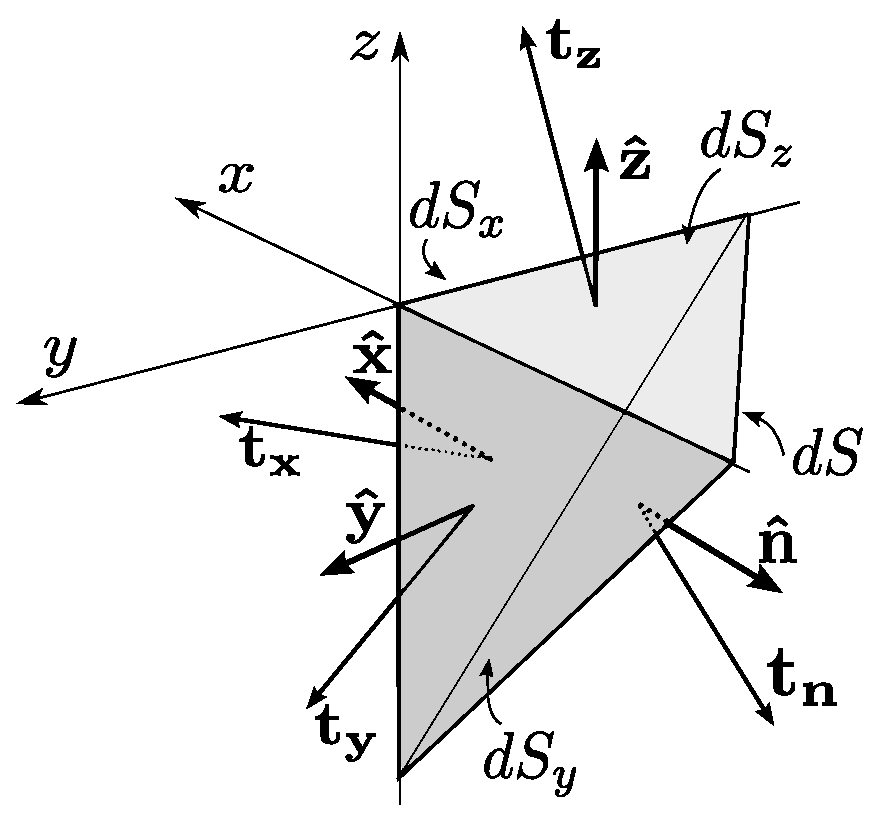
\includegraphics[width=0.60\textwidth]{./fig/cauchy.eps}
\caption{tetraedro di Cauchy}\label{fig:tetraedroCauchy}
\end{figure}

\begin{example}[Tensore di inerzia] Durante il corso di Meccanica Razionale si è visto che le componenti del tensore di inerzia espresse in un sistema di riferimento cartesiano ortogonale possono essere raccolte nella matrice simmetrica,
\begin{equation}
 \int_V \rho
 \begin{bmatrix}
   (y^2+z^2) &     -xy    &    -xz     \\ 
      -xy    &  (x^2+z^2) &    -yz     \\ 
      -xz    &     -yz    &  (x^2+y^2) \\ 
 \end{bmatrix}
\end{equation}
\begin{exercise}[Espressione tensoriale del tensore di inerzia] 
   Aiutandosi con un sistema di riferimento cartesiano, si dimostri che l'espressione tensoriale del tensore di inerzia è
    \begin{equation}
      \mathbb{I}_G = \int_V \rho \left[ |\bm{r}|^2 \mathbb{I} 
         - \bm{r} \otimes \bm{r} \right] \ ,
    \end{equation}
    essendo $\mathbb{I}$ il tensore identità del secondo ordine, $\bm{r}$ il raggio vettore tra un punto del corpo considerato e il punto $G$ rispetto al quale si sta calcolando il tensore di inerzia e l'integrale viene svolto su tutto il volume $V$ del corpo.
\end{exercise}
\end{example}

\begin{exercise}
    Dato il tensore simmetrico del secondo ordine definito nella base ortonormale $\{\bm{\hat{x}}, \bm{\hat{y}}\}$ dello spazio bidimensionale,
\begin{equation}
    \mathbb{A} = A_{xx} \bm{\hat{x}} \otimes \bm{\hat{x}} +
                 A_{xy} \bm{\hat{x}} \otimes \bm{\hat{y}} +
                 A_{xy} \bm{\hat{y}} \otimes \bm{\hat{x}} +
                 A_{yy} \bm{\hat{y}} \otimes \bm{\hat{y}} \ ,
\end{equation}
 si chiede di determinare la base ortonormale $\{\bm{\hat{\xi}},\bm{\hat{\eta}}\}$, che consente di esprimere il tensore $\mathbb{A}$ come 
\begin{equation}
    \mathbb{A} = A_{\xi \xi } \bm{\hat{\xi }} \otimes \bm{\hat{\xi }} +
                 A_{\eta\eta} \bm{\hat{\eta}} \otimes \bm{\hat{\eta}} \ , 
\end{equation}
cioé in forma diagonale.
\end{exercise}
%
\begin{figure}[h]
 \centering
 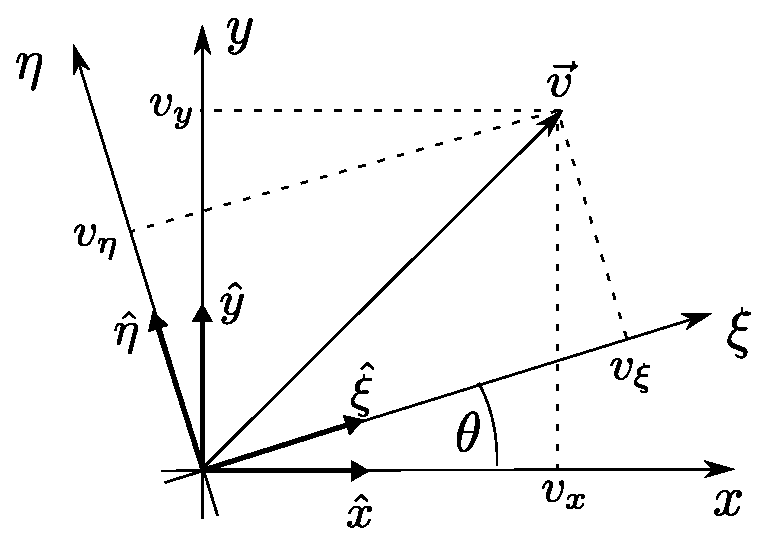
\includegraphics[width=0.5\textwidth]{./fig/rotation}
    \caption{Cambio di base: basi ortonormali.}\label{fig:tensor:rotation}
\end{figure}
Dati i due sistemi di riferimento raffigurati in figura \ref{fig:tensor:rotation}, la legge di trasformazione tra i vettori delle due basi è
\begin{equation}
 \begin{cases}
   \bm{\hat{\xi}} =  \cos{\theta} \bm{\hat{x}} + \sin{\theta} \bm{\hat{y}} \\
   \bm{\hat{\eta}} = -\sin{\theta} \bm{\hat{x}} + \cos{\theta} \bm{\hat{y}} \
 \end{cases} \qquad \rightarrow \qquad
    [ \bm{\hat{\xi}} | \bm{\hat{\eta}} ] = [ \bm{\hat{x}} | \bm{\hat{y}} ] \ T
\end{equation}
avendo indicato con $T$ la trasformazione lineare
\begin{equation}
 T = 
\begin{bmatrix}
 \cos{\theta} & \sin{\theta} \\
-\sin{\theta} & \cos{\theta} 
\end{bmatrix} \ ,
\end{equation}
e definendo $\tilde{T}=T^{-1}=T^T$, la sua inversa. Utilizzando la formula (\ref{eqn:t2t:t}), la trasformazione delle componenti di un tensore del secondo ordine diventa
\begin{equation}
    \tilde{A}_{ik} = \tilde{T}_{il} \tilde{T}_{km} A_{lm} \qquad , \qquad
    \tilde{A} = \tilde{T} A \tilde{T}^T \ ,
\end{equation}
non avendo fatto distinzione tra pedici e indici poiché si usano due basi ortonormali.
Si può quindi esplicitare l'ultima espressione per ricavare l'espressione delle componenti del tensore $\mathbb{A}$ nel nuovo sistema di riferimento,
 \begin{equation}
   \begin{bmatrix}
    A_{\xi \xi} & A_{\xi \eta} \\
    A_{\eta\xi} & A_{\eta\eta} \\
   \end{bmatrix} = 
   \begin{bmatrix} 
    \cos{\theta} & \sin{\theta} \\
   -\sin{\theta} & \cos{\theta} \\
   \end{bmatrix}
   \begin{bmatrix}
    A_{xx} & A_{xy} \\
    A_{yx} & A_{yy} \\
   \end{bmatrix}
   \begin{bmatrix} 
    \cos{\theta} &-\sin{\theta} \\
   \sin{\theta} & \cos{\theta} \\
   \end{bmatrix}
 \end{equation}
Svolgendo i conti e sfruttando la simmetria del tensore $\mathbb{A}$, $A_{xy} = A_{yx}$, si ottiene
  \begin{equation}
  \begin{aligned}
& \begin{bmatrix}
    A_{\xi \xi} & A_{\xi \eta} \\
    A_{\eta\xi} & A_{\eta\eta} \\
   \end{bmatrix} = \\ 
   & = \begin{bmatrix}
    A_{xx} \cos^2 \theta + A_{yy} \sin^2 \theta + 2 A_{xy} \cos \theta \sin \theta & 
      (-A_{xx} + A_{yy}) \cos \theta \sin \theta + A_{xy} ( \cos^2 \theta - \sin^2 \theta) \\
  (-A_{xx} + A_{yy}) \cos \theta \sin \theta + A_{xy} ( \cos^2 \theta - \sin^2 \theta) &
      A_{xx} \sin^2 \theta + A_{yy} \cos^2 \theta - 2 A_{xy} \cos \theta \sin \theta 
   \end{bmatrix} \ .
 \end{aligned}
 \end{equation}
Si osservi che la proprietà di simmetria del tensore è indipendente dalla base ortonormale utilizzata per esprimerne le componenti, $A_{\xi \eta} = A_{\eta \xi}$.
Per trovare l'angolo $\theta$ del quale bisogna ruotare il sistema di riferimento $\{\bm{\hat{\xi}},\bm{\hat{\eta}} \}$ affinché la componente $A_{\xi \eta}$ sia nulla, si impone
  \begin{equation}
   A_{\xi \eta} = 0 \ ,
  \end{equation}
ottenendo
  \begin{equation}
   0 = A_{xy} \cos {2\theta} - \dfrac{\sin{2\theta}}{2} (A_{xx}-A_{yy}) \quad \Rightarrow \quad
   \tan {2 \theta} = \dfrac{2 A_{xy}}{A_{xx}-A_{yy}} \ .
  \end{equation}
 %
 Il problema oggetto di questo esercizio è equivalente alla ricerca degli \textbf{assi principali di sforzo} per uno stato di sforzo piano, coincidenti con gli \textbf{autovettori} del tensore.\footnote{
     Gli autovettori di un tensore del secondo ordine $\mathbb{A}$ possono essere definiti come quei vettori $\bm{v}$ per i quali vale $\mathbb{A} \cdot \bm{v} = \lambda \bm{v}$ (autovettori ``destri'') oppure $\bm{v} \cdot \mathbb{A} = \lambda \bm{v}$ (autovettori ``sinistri''). Si ricorda che autovettori destri e sinistri coincidono nel caso in cui il tensore sia simmetrico. Infatti le due espressioni
\begin{equation}
\begin{aligned}
    \bm{v} \cdot \mathbb{A} & = v_i \bm{b}^i \cdot A^{jk} \bm{b}_j \otimes \bm{b}_k = 
    v_i A^{ik} \bm{b}_k \\
    \mathbb{A} \cdot \bm{v} & = A^{ij} \bm{b}_i \otimes \bm{b}_j \cdot v_k \bm{b}^k  = 
    A^{ij} v_j \bm{b}_i = A^{ki} v_i \bm{b}_k \ ,
\end{aligned}
\end{equation}
coincidono quando $A^{ij} = A^{ji}$. Nell'ultimo passaggio sono state modificate le lettere che identificano gli indici ripetuti per rendere più evidente il confronto tra le due espressioni.
Si ricorda inoltre che gli autovettori (opportunamente normalizzati) di un tensore simmetrico formano una base ortonormale $\{ \bm{v}^{(1)} , \dots , \bm{v}^{(N)} \}$, che può essere utilizzata per scrivere il tensore tramite la sua decomposizione spettrale
\begin{equation}
 \mathbb{A} = \lambda^{(1)} \bm{v}^{(1)} \otimes \bm{v}^{(1)} + \dots
              \lambda^{(N)} \bm{v}^{(N)} \otimes \bm{v}^{(N)} \ ,
\end{equation}
essendo $\lambda^{(i)}$ gli autovalori associati agli autovettori. Per convincersi della validità di tale decomposizione, è sufficiente moltiplicare con il ``prodotto punto'' il tensore $\mathbb{A}$ per uno dei vettori della base. Moltiplicandolo ad esempio per $\bm{v}^{(i)}$ e sfruttando l'ortogonalità dei vettori della base, si ottiene
\begin{equation}
\begin{aligned}
    \mathbb{A} \cdot \bm{v}^{(i)} & =
    \sum_{k=1}^{N} \left( \lambda^{(k)} \bm{v}^{(k)} \otimes \bm{v}^{(k)} \right) \cdot \bm{v}^{(i)}  = \\
& = \sum_{k=1}^{N} \left( \lambda^{(k)} \bm{v}^{(k)} \delta^{ik}\right) = 
    \lambda^{(i)} \bm{v}^{(i)} \ .
\end{aligned}
\end{equation}
 }
  Il risultato ricavato tramite le trasformazioni delle componenti dei tensori coincide con quello  già ottenuto nei corsi precedenti tramite l'equilibrio di un elementino di materiale, riassumibile nel diagramma del cerchio di Mohr. Avere in mente entrambi gli approcci può essere utile per non perdere il significato fisico di quello che si sta facendo.
%
\newline \noindent 
 La trasformazione delle componenti di un tensore in seguito al cambio di base può trovare molte altre applicazioni: un'altra applicazione ``da strutturista'' un po' più avanzato, consiste la determinazione delle caratteristiche meccaniche di elementi strutturali in materiale in composito, partendo dalle proprietà delle lamine che vengono usate per costruirlo.
 Ogni lamina ha caratteristiche meccaniche facilmente descrivibili nel proprio sistema di riferimento, la cui orientazione è determinata dalla direzione delle fibre, ad esempio, e che in generale è diversa da lamina a lamina. Le caratteristiche meccaniche del elemento strutturale vengono infine espresse in un suo sistema di riferimento globale, definito ad esempio dalla geometria del componente. 
%
\newline \noindent 
 Queste poche righe non hanno pretese di completezza, ma vogliono attirare l'interesse su quanto abbiamo visto nelle ultime ore, anche da parte di quelli che diventeranno ``strutturisti'' ma non solo.

\clearpage \newpage

\subsection{Cosa non è stato detto}
 Molte cose non sono state dette. Innanzitutto si è scelto di limitarsi alla rappresentazione di vettori e tensori utilizzando basi ortonormali dello spazio. Inoltre, è stato scelto di trattare i tensori su spazi forniti di prodotto interno e di non introdurre concetti di \textit{algebra esterna}, che permetterebbero di generalizzare l'operazione di prodotto vettoriale e l'operatore rotore incontrato nel calcolo vettoriale e ricavare il teorema di Stokes,
\begin{equation}
 \oint_{\partial \Omega} \omega = \int_\Omega d\omega ,
\end{equation}
 di cui viene solo riportata l'espressione matematica senza fornire alcun dettaglio. Il teorema del rotore e della divergenza sono casi particolari del teorema di Stokes, nel cui enunciato compaiono i concetti di forma differenziale $\omega$ e di derivata esterna $d \omega$.

 \noindent
Il materiale fornito rappresenta un compromesso tra il vuoto totale sul calcolo tensoriale (del quale l'affermazione ``un tensore è una matrice'' è la regina indiscussa) e un corso intero dedicato all'algebra e al calcolo tensoriale. Lo scopo dei cenni veloci ad argomenti non trattati qui è quello di ``mettere una pulce nell'orecchio'' di chi legge, di mettere a conoscenza il lettore dell'esistenza di alcuni argomenti che permettono di generalizzare le operazioni vettoriali presentate nei primi corsi di Algebra e di spiegare in maniera rigorosa alcuni comportamenti strani o inaspettati (come quelli che si possono osservare con il prodotto vettoriale e il rotore), senza scoperchiare dei vasi di Pandora che porterebbero questa introduzione lontana dal suo scopo.

\vspace{10pt}
 \noindent
 Per i più curiosi, viene messo a disposizione del materiale un più completo, che introduce concetti che non sono stati presentati qui e che generalizzano la trattazione, ma che la renderebbero inadatta ad essere svolta in poche ore per un pubblico formato da studenti del terzo anno di ingegneria, senza aggiungere particolari fondamentali per un utilizzo ``cosciente'' dei tensori durante questo corso e in quelli successivi.

 \subsubsection{Riferimenti.}  
 Il testo di Bowen e Wang, \textit{Introduction to vectors and tensors. Linear and multilinear algebra} può essere considerato un valido e completo riferimento, anche per il futuro. La lettura di questo testo non è sempre agevole e contiene sicuramente molto più di quanto sia indispensabile presentare in una prima e breve introduzione ai tensori, come è questa.
 Oltre alla sua qualità, è da apprezzare la disponibilità in rete dei due volumi, seguendo i seguenti collegamenti (sperando che siano ancora validi):
 
 \href{http://oaktrust.library.tamu.edu/bitstream/handle/1969.1/2502/IntroductionToVectorsAndTensorsVol1.pdf}
 {Vol. 1: Linear and Multilinear Algebra}
 
 \href{http://oaktrust.library.tamu.edu/bitstream/handle/1969.1/3609/IntroductionToVectorsAndTensorsVol2.pdf}
 {Vol. 2: Vector and Tensor Analysis}
 
% http://www.mat.unimi.it/users/carati/didattica/dispense/tensori.pdf
 
 
 \subsubsection{Cosa è utile ripassare.} Questa può essere una buona occasione per ripassare alcuni concetti di algebra lineare, tra i quali quello di spazio vettoriale (definizione e proprietà, dimensione e base, \dots), prodotto interno, linearità (e la differenza con l'essere ``affine''), alla luce di quanto visto in questi paragrafi introduttivi sui tensori e del fatto che le equazioni della fisica hanno carattere tensoriale.




